\chapter{Analisi dei Requisiti}

\subsection*{Requisiti Utente}
L'obiettivo di questo capitolo è definire le iterazioni tra gli attori e il sistema software, al fine di mappare i requisiti funzionali emersi in fase di analisi. Questo ci permette di descrivere il comportamento del sistema dal punto di vista dell'utente. \\
Di seguito vengono descritti i principali casi d'uso, strutturati secondo i principi del manifesto per lo Sviluppo Agile di Software. 

\section{Use Case Utente Registrato (Cittadino)}
Di seguito vengono analizzati i principali casi d'uso relativi all'Utente Registrato. \\
\`E presente un diagramma dei casi d'uso (UML), pensato per fornire una visione d'insieme del sistema.
In seguito, è presente la documentazione tecnica, che include descrizioni dettagliate e tabelle strutturate che analizzano le singole operazioni definite nel diagramma del caso d'uso.

\vspace{0.5cm}

\subsection*{Diagramma}
\addcontentsline{toc}{subsection}{Diagramma}
\begin{figure}[H]
    \centering
    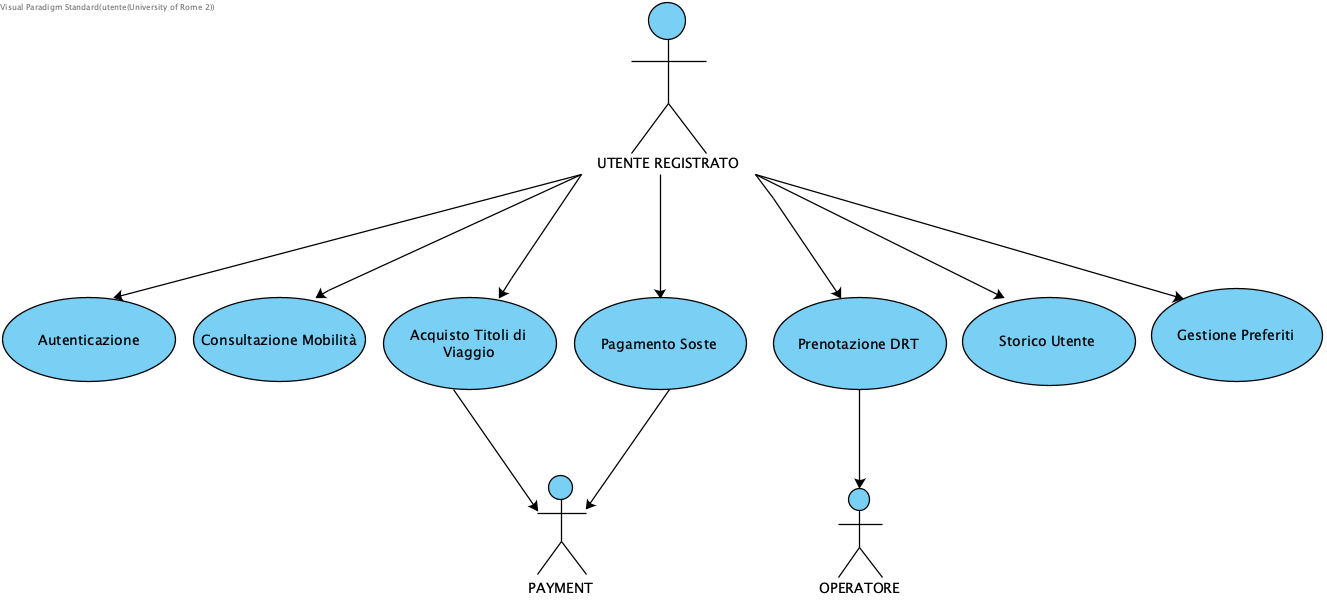
\includegraphics[width=0.9\linewidth]{UseCase/Utente_Registrato.png}
    \label{fig:placeholder}
\end{figure}
\newpage

\subsection*{Documentazione}
\addcontentsline{toc}{subsection}{Documentazione}

\begin{center}
    Use Case: Autenticazione. 
\end{center}
Il caso d'uso Autenticazione, descrive la procedura di accesso al sistema da parte dell'Utente Registato. \\
Attraverso l'autenticazione il sistema ricorda chi è l'utente, in base ai dati che ha fornito durante la Registrazione. \\
Tramite l'inserimento delle proprie credenziali, l'utente viene riconosciuto dal sistema e sblocca servizi avanzati appositamente per lui, ovvero consultare i suoi titoli di viaggio o i suoi abbonamenti, la sua cronologia, e così via.  

\vspace{0.5cm}

%TABELLA 
\usecasetable
{Autenticazione}
{Procedura di accesso al sistema tramite verifica delle credenziali.}
{Utente Registrato, Admin, Operatore, Funzionario.}
{L'utente deve possedere un account attivo.}
{1. L'utente inserisce email e password. \newline 2. Il sistema valida i dati. \newline 3. Viene garantito l'accesso al profilo.}
{1a. Credenziali errate: il sistema segnala l'errore e nega l'accesso.}
{Sessione utente avviata e accesso alle funzionalità riservate.}
\newpage
\begin{center}
    Use Case: Consultazione mobilità. 
\end{center}
Il caso d'uso Consultazione Mobilità, condiviso dai profili Turista e Utente non Registrato, consente la ricerca e la visualizzazione di informazioni relative alla rete di trasporto, permettendo all'Utente Registrato la consultazione di percorsi, orari, tratte e fermate con aggiornamenti in tempo reale. 

\vspace{0.5cm}

%TABELLA 
\usecasetable
{Consultazione mobilità}
{Ricerca di informazioni su tratte, orari e fermate con dati real-time.}
{Utente Registrato, Non Registrato, Turista.}
{Connessione al server attiva.}
{1. L'utente cerca una tratta. \newline 2. Il sistema mostra orari e percorsi disponibili.}
{1a. Dati in tempo reale non disponibili: il sistema mostra l'orario programmato.}
{Visualizzazione delle informazioni di viaggio.}
\newpage

\begin{center}
    Use Case: Acquisto Titoli di Viaggio
\end{center}
Il caso d'uso Acquisto Titoli di Viaggio consente l'acquisto di biglietti per le diverse tratte della rete. Questa funzionalità è prevista anche per il profilo Turista, ma è strettamente subordinata al completamento delle procedure di registrazione e autenticazione, configurandosi di fatto come un'azione riservata all'Utente che effettua l'autenticazione. 

\vspace{0.5cm}

%TABELLA
\usecasetable
{Acquisto Titoli di Viaggio}
{Acquisto di biglietti o abbonamenti digitali.}
{Utente Registrato, Turista, Payment.}
{Utente autenticato nel sistema.}
{1. Selezione titolo. \newline 2. Reindirizzamento al pagamento. \newline 3. Conferma transazione.}
{2a. Transazione fallita: il sistema annulla l'ordine e avvisa l'utente.}
{Titolo di viaggio disponibile nel profilo utente.}

\begin{center}
    Use Case: Prenotazione DRT.
\end{center}
Il caso d'uso Prenotazione DRT, condiviso anch'esso con il profilo del Turista, è un'azione riservata all'Utente che effettua l'autenticazione. Permette all'Utente Registrato di usufruire dei servizi \textit{Demand Responsive Transport (DRT)}, ovvero il trasporto su richiesta basato su corse a chiamata per collegare le frazioni al centro urbano durante specifiche fasce orarie. 

\vspace{0.5cm}

% TABELLA 
\usecasetable
{Prenotazione DRT}
{Richiesta di trasporto a chiamata per frazioni periferiche.}
{Utente Registrato, Turista, Operatore.}
{Utente autenticato.}
{1. Richiesta corsa. \newline 2. Accettazione dell'Operatore. \newline 3. Conferma orario.}
{2a. Rifiuto corsa: l'operatore segnala indisponibilità.}
{Corsa prenotata e inserita nell'agenda dell'operatore.}
\newpage

\begin{center}
    Use Case: Gestione preferiti
\end{center}
Il caso d'uso Gestione Preferiti consente all'utente di memorizzare i percorsi e le fermate di maggiore interesse, oltre a mantenere traccia dello storico delle transazioni passate. Questo caso d'uso è accessibile anche al profilo Turista, dopo aver effettuato il completamento delle procedure di registrazione e autenticazione.

\vspace{0.5cm}

% TABELLA 
\usecasetable
{Gestione Preferiti}
{Salvataggio e organizzazione di percorsi, fermate e tratte frequenti.}
{Utente Registrato, Turista.}
{Utente autenticato nel sistema.}
{1. Selezione di un elemento (fermata/tratta). \newline 2. Comando "Aggiungi ai preferiti". \newline 3. Conferma dell'inserimento nel profilo.}
{2a. Elemento già presente: il sistema propone la rimozione o l'aggiornamento dell'etichetta.}
{L'elemento è disponibile nella sezione "Preferiti" per un accesso rapido.}

\begin{center}
    Use Case: Storico Utente
\end{center}
Il caso d'uso Storico Utente, anch'esso condiviso con il profilo Turista, azione accessibile solo dopo aver effettuata la registrazione e l'autenticazione. Consente all'Utente Registrato di visualizzare l'elenco dei viaggi effettuati dalle transizioni passate. 

\vspace{0.5cm}

% TABELLA 
\usecasetable
{Storico Utente}
{Consultazione dell'elenco dei viaggi effettuati e delle transazioni passate.}
{Utente Registrato, Turista.}
{Utente autenticato nel sistema.}
{1. Accesso all'area personale. \newline 2. Selezione sezione "Storico". \newline 3. Visualizzazione dettagli viaggi e ricevute.}
{1a. Storico vuoto: il sistema visualizza un messaggio di assenza di dati.}
{L'utente ottiene visibilità sulle proprie attività pregresse.}
\newpage

\section{Use Case Utente Non Registrato}
Di seguito vengono analizzati i principali casi d'uso relativi all'Utente non Registrato.
\\
Ciascuna descrizione è seguita dal relativo diagramma dei casi d'uso (UML), pensato per fornire una visione d'insieme, e seguita dalla documentazione tecnica, che include tabelle strutturate per analizzare nel dettaglio le singole operazioni. 

\vspace{0.5cm}

\subsection*{Diagramma}
\addcontentsline{toc}{subsection}{Diagramma}
\begin{figure}[H]
    \centering
    \includegraphics[width=0.6\linewidth]{UseCase/Utente_non_Registrato.png}
    \label{fig:placeholder}
\end{figure}

\subsection*{Documentazione}
\addcontentsline{toc}{subsection}{Documentazione}

\begin{center}
    Use Case: Registrazione. 
\end{center}
Il caso d'uso Registrazione, descrive la procedura di accesso al sistema da parte dell'Utente non Registato. \\
Quest'ultimo deve registrarsi al sistema affinchè possa usare funzionalità e servizi aggiuntivi. \\
Per Registrarsi si necessita dell'inserimento dei seguenti dati: Nome, Cognome, Codice Fiscale (Identificativo), Residenza, Tipologia (Cittadino o Turista), e così via. 

\vspace{0.5cm}

%TABELLA 
\usecasetable
{Registrazione}
{Creazione di un nuovo profilo utente nel sistema.}
{Utente Non Registrato.}
{Disponibilità di una connessione di rete e dati anagrafici validi.}
{1. Inserimento dati (Nome, CF, Residenza). \newline 2. Invio richiesta. \newline 3. Validazione, creazione account e assegnazione tipologia account}
{1a. Utente già esistente: il sistema segnala che il Codice Fiscale è già censito.}
{Creazione del profilo e abilitazione alle funzionalità per Utente Registrato.}

\begin{center}
    Use Case: Consultazione mobilità. 
\end{center}
Il caso d'uso Consultazione Mobilità, condiviso dai profili Turista e Utente Registrato, consente la ricerca e la visualizzazione delle informazioni di base inerenti alla rete di trasporto. Nello specifico, per il solo Utente Registrato, il sistema offre un livello di accesso avanzato che include la consultazione dettagliata di percorsi, orari, tratte e fermate, integrando aggiornamenti sul servizio in tempo reale.

\vspace{0.5cm}

%TABELLA 
\usecasetable
{Consultazione Mobilità}
{Ricerca di informazioni generiche sulla rete di trasporto senza autenticazione.}
{Utente Non Registrato.}
{Nessuna.}
{1. Accesso alla home page. \newline 2. Ricerca orari o linee. \newline 3. Visualizzazione risultati pubblici.}
{1a. Servizio offline: il sistema mostra l'ultimo aggiornamento disponibile in cache.}
{Informazioni ottenute senza persistenza dei dati di ricerca.}
\newpage

\section{Use Case Turista}
Di seguito è riportata l'analisi dei principali casi d'uso che coinvolgono il profilo del Turista. \\ 
Ciascuna descrizione è fornita dal rispettivo diagramma (UML), che fornisce una visione d'insieme delle azioni, e dalla documentazione tecnica strutturata per un'analisi dettagliata delle operazioni.

\subsection*{Diagramma}
\addcontentsline{toc}{subsection}{Diagramma}
\begin{figure}[H]
    \centering
    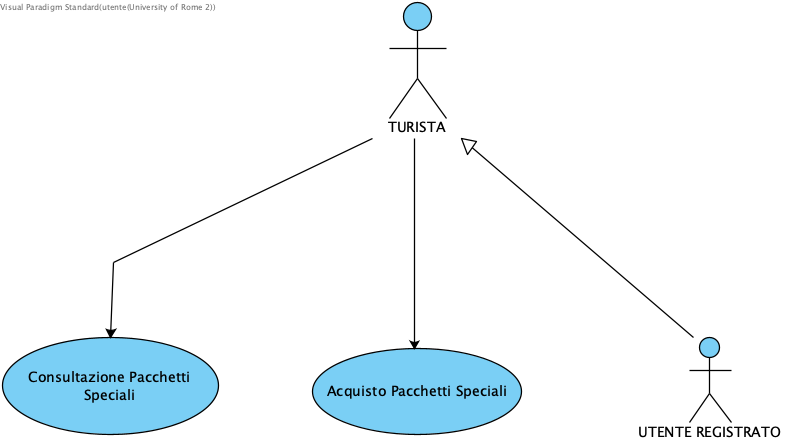
\includegraphics[width=0.7\linewidth]{UseCase/Turista.png}
    \label{fig:placeholder}
\end{figure}

\subsection*{Documentazione}
\addcontentsline{toc}{subsection}{Documentazione}

\begin{center}
    Use Case: Consultazione Pacchetti Speciali. 
\end{center}
Il caso d'uso Consultazione di Pacchetti Speciali, solamente relativo al profilo del Turista. Anch'esso vincolato al completamento delle procedure di registrazione e autenticazione. Consente al Turista di accedere  e consultare biglietti o Pacchetti Speciali per effettuare i vari spostamenti all'interno e all'esterno del comune. 

\vspace{0.5cm}

%TABELLA 
\usecasetable
{Consultazione Pacchetti Speciali}
{Visualizzazione di offerte integrate per la mobilità turistica.}
{Turista.}
{Utente autenticato come profilo "Turista".}
{1. Accesso sezione "Offerte". \newline 2. Filtro per durata o zona. \newline 3. Visualizzazione dettagli pacchetto.}
{2a. Nessun pacchetto attivo: il sistema mostra le tariffe standard.}
{Conoscenza delle opzioni di risparmio per visitatori.}
\newpage

\begin{center}
    Use Case: Acquisto Pacchetti Speciali.
\end{center}
Il caso d'uso Acquisto di Pacchetti Speciali, inerente solamente al profilo del Turista. Anch'esso vincolato al completamento delle procedure di registrazione e autenticazione. Permette al Turista di accedere ed acquistare biglietti o Pacchetti Speciali per effettuare i vari spostamenti all'interno e all'esterno del comune. 

\vspace{0.5cm}

%TABELLA 
\usecasetable
{Acquisto Pacchetti Speciali}
{Transazione economica per l'attivazione di un bundle di servizi turistici.}
{Turista, Payment.}
{Utente autenticato e metodo di pagamento valido.}
{1. Selezione pacchetto. \newline 2. Procedura di check-out. \newline 3. Validazione pagamento e attivazione.}
{3a. Errore Gateway: il sistema annulla l'operazione e ripristina lo stato precedente.}
{Pacchetto turistico associato digitalmente al profilo dell'utente.}
\newpage

\section{Use Case Admin Dell'Ente}
Passiamo ora all'analisi dei casi d'uso che riguardano l'Admin Ente. \\
Qui è presente il diagramma UML, che aiuta ad avere subito un'idea chiara delle funzionalità. \\
Subito dopo si trova la documentazione tecnica, dove attraverso delle tabelle vengono spiegate passo passo le singole operazioni.

\subsection*{Diagramma}
\addcontentsline{toc}{subsection}{Diagramma}
\begin{figure}[H]
    \centering
    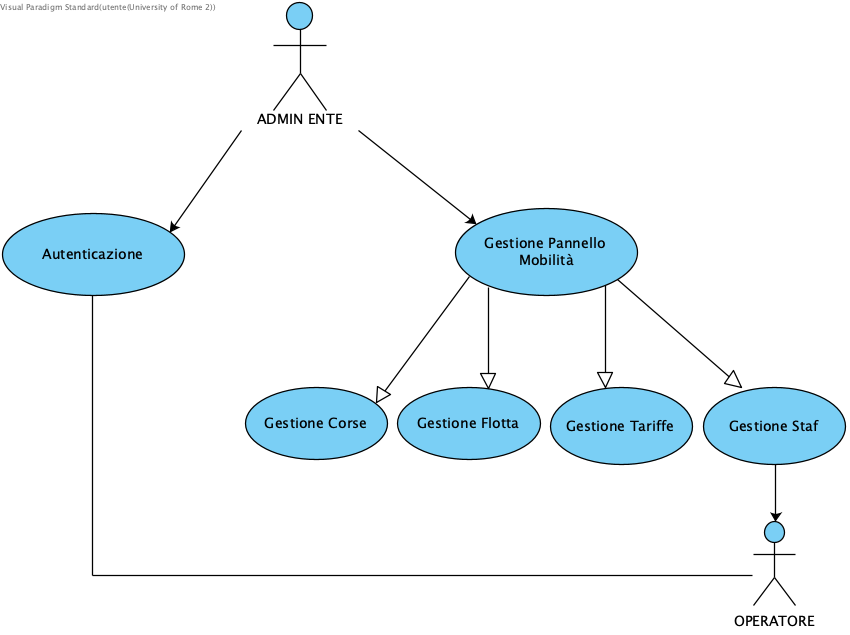
\includegraphics[width=0.7\linewidth]{UseCase/Admin_Ente.png}
    \label{fig:uc_admin_ente}
\end{figure}

\subsection*{Documentazione}
\addcontentsline{toc}{subsection}{Documentazione}

\begin{center}
    {Use Case: Autenticazione}
\end{center}
Il caso d'uso Autenticazione descrive la procedura di accesso al sistema da parte dell'Admin dell'Ente. \\
Attraverso l'autenticazione il sistema ricorda chi è l'admin, in base ai dati che ha fornito durante la Registrazione. \\
Tramite l'inserimento delle proprie credenziali, l'utente viene riconosciuto dal sistema e sblocca servizi avanzati appositamente per lui. Ovvero gestire le corse, vedere i guadagni e monitorare i mezzi.

\vspace{0.5cm}

%TABELLA
\usecasetable
{Autenticazione Admin}
{Accesso protetto al backend di gestione dell'Ente.}
{Admin Ente.}
{Possesso di credenziali amministrative.}
{1. Inserimento credenziali. \newline 2. Verifica credenziali. \newline 3. Accesso al pannello di controllo.}
{1a. Accesso negato: segnalazione di tentativo non autorizzato.}
{Accesso completo alle funzioni di configurazione sistema.}

\begin{center}
    {Use Case: Gestione Pannello Mobilità}
\end{center}
Il caso d'uso Gestione Pannello Mobilità, rappresenta l'hub centrale a cui l'Admin Ente ha accesso. Da questo pannello si diramano le funzionalità specifiche di amministrazione (corse, flotta, tariffe e staff), che costituiscono una specializzazione delle operazioni di mobilità.

\vspace{0.5cm}

%TABELLA
\usecasetable
{Gestione Pannello Mobilità}
{Hub centrale per l'amministrazione e la specializzazione delle operazioni di mobilità (corse, flotta, tariffe e staff).}
{Admin Ente.}
{L'Admin Ente deve aver effettuato l'accesso al sistema (Autenticazione completata con successo).}
{1. L'Admin accede alla dashboard principale. \newline 2. Il sistema mostra la panoramica dei servizi di mobilità. \newline 3. L'Admin seleziona l'area di interesse (es. gestione corse o flotta).}
{2a. Errore di caricamento dati: il sistema mostra un avviso e tenta una riconnessione al database.}
{L'Admin viene reindirizzato alla sezione specifica selezionata, pronto per eseguire operazioni di CRUD (Creazione, Lettura, Aggiornamento, Cancellazione).}
\newpage

\begin{center}
    {Use Case: Gestione Corse}
\end{center}
Il caso d'uso Gestione Corse, relativo solamente al profilo dell'Admin dell'Ente, permette l'inserimento delle tratte che saranno visibili all'interno del sistema.

\vspace{0.5cm}

%TABELLA
\usecasetable
{Gestione Corse}
{Modifica e programmazione delle tratte di trasporto ordinario.}
{Admin Ente.}
{Autenticazione Admin completata.}
{1. Selezione linea. \newline 2. Modifica orari o fermate. \newline 3. Pubblicazione variazioni.}
{3a. Conflitto di orari: il sistema segnala la sovrapposizione di mezzi sulla stessa tratta.}
{Database delle corse aggiornato in tempo reale per gli utenti.}

\vspace{0.5cm}

\begin{center}
    {Use Case: Gestione Flotta}
\end{center}
Il caso d'uso Gestione Flotta, anch'esso relativo solamente al profilo dell'Admin dell'Ente, permette la gestione dei mezzi, ovvero l'inserimento o la rimozione dei veicoli ad uso del Comune.

\vspace{0.5cm}

%TABELLA
\usecasetable
{Gestione Flotta}
{Amministrazione dei mezzi fisici (bus, navette) in dotazione.}
{Admin Ente.}
{Autenticazione Admin completata.}
{1. Schedatura nuovo mezzo o rimozione esistente. \newline 2. Associazione mezzo a linea. \newline 3. Salvataggio.}
{1a. ID Mezzo duplicato: il sistema richiede una matricola univoca.}
{Anagrafica flotta aggiornata e sincronizzata con la disponibilità operativa.}
\newpage

\begin{center}
    {Use Case: Gestione Tariffe}
\end{center}
Il caso d'uso Gestione Tariffe, anch'esso relativo solamente al profilo dell'Admin dell'Ente, permette all'Ente di gestire le Tariffe, consultare le entrate e le uscite, e i rimborsi.

\vspace{0.5cm}

% TABELLA
\usecasetable
{Gestione Tariffe}
{Configurazione dei prezzi e monitoraggio finanziario.}
{Admin Ente.}
{Autenticazione Admin completata.}
{1. Accesso modulo tariffe. \newline 2. Modifica prezzi o gestione rimborsi. \newline 3. Salvataggio.}
{1a. Errore dati: il sistema blocca il salvataggio di valori incongrui.}
{Parametri tariffari aggiornati nel database.}

\vspace{0.5cm}

\begin{center}
    {Use Case: Gestione Staff}
\end{center}
Il caso d'uso Gestione Staff, anch'esso relativo solamente all'Admin dell'Ente, permette la gestione degli operatori dei bus, dei controllori e di coloro che sono dipendenti dell'Ente e si trovano nella gestione dei trasporti del comune. Il sistema prevede anche un'interazione diretta con il profilo dell'Operatore, che esegue le direttive assegnate.

\vspace{0.5cm}

% TABELLA
\usecasetable
{Gestione Staff}
{Amministrazione del personale (autisti, controllori).}
{Admin Ente.}
{Autenticazione Admin completata.}
{1. Selezione dipendente. \newline 2. Assegnazione ruolo o turno. \newline 3. Aggiornamento anagrafica.}
{1a. Dipendente già assegnato: il sistema segnala il conflitto di turnazione.}
{Organico aziendale aggiornato.}
\newpage

\section{Use Case Operatore}
In questa sezione ci concentriamo sull'Operatore. \\ Anche in questo caso, è presente un diagramma UML per dare una visione d'insieme del processo. \\ A seguire, sono state riportate le tabelle tecniche per scendere nel dettaglio di come funziona esattamente ogni azione.

\subsection*{Diagramma}
\addcontentsline{toc}{subsection}{Diagramma}
\begin{figure}[H]
    \centering
    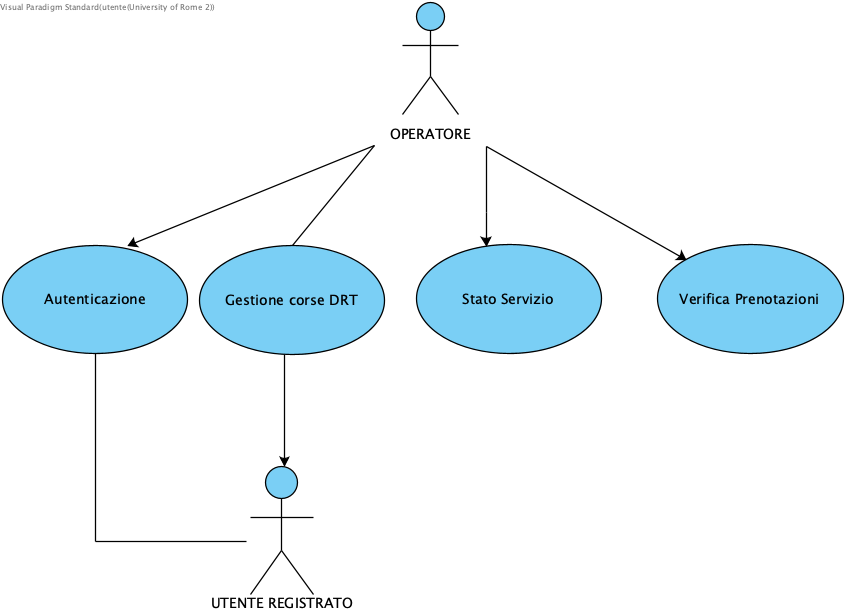
\includegraphics[width=0.7\linewidth]{UseCase/Operatore.png}
    \label{fig:placeholder}
\end{figure}

\subsection*{Documentazione}
\addcontentsline{toc}{subsection}{Documentazione}

\begin{center}
    Use Case: Autenticazione. 
\end{center}
Il caso d'uso Autenticazione, descrive la procedura di accesso al sistema da parte dell'Operatore. \\
Attraverso l'autenticazione il sistema ricorda chi è l'operatore, in base ai dati che ha fornito durante la Registrazione. \\
Tramite l'inserimento delle proprie credenziali, l'utente viene riconosciuto dal sistema e sblocca servizi appositamente per lui.

\vspace{0.5cm}

%TABELLA 
\usecasetable
{Stato Servizio}
{Aggiornamento della condizione operativa dei mezzi (in ritardo, guasto, attivo).}
{Operatore.}
{Operatore autenticato e in turno.}
{1. Selezione mezzo/corsa. \newline 2. Cambio stato (es. "In ritardo"). \newline 3. Invio aggiornamento al sistema.}
{2a. Errore di connessione: salvataggio locale e tentativo di reinvio automatico.}
{Informazione distribuita in tempo reale a tutti gli utenti del sistema.}

\begin{center}
    Use Case: Gestione Corse DRT. 
\end{center}
Il caso d'uso Gestione Corse DRT, solamente relativo al proflo dell'Operatore, permette la visione delle chiamate da parte dell'Utente Registrato o del Turista.\\  L'Operatore non solo riceve la chiamata, ma sceglie se accettare o meno la partenza della corsa.

\vspace{0.5cm}

%TABELLA 
\usecasetable
{Gestione Corse DRT}
{Validazione delle richieste di trasporto su chiamata.}
{Operatore.}
{Autenticazione Operatore completata.}
{1. Ricezione notifica chiamata. \newline 2. Valutazione logistica. \newline 3. Accettazione o rifiuto.}
{2a. Mezzi insufficienti: l'operatore declina la richiesta.}
{Aggiornamento dello stato della prenotazione lato utente.}
\newpage

\begin{center}
    Use Case: Stato Servizio.
\end{center}
Il caso d'uso Stato Servizio, anch'esso solamente relativo al profilo dell'Operatore, permette la gestione dei mezzi e degli orari, ovvero l'inserimento o l'attivazione della partenza dei mezzi disponibili.

\vspace{0.5cm}

%TABELLA 
\begin{table}[htbp]
\centering
\renewcommand{\arraystretch}{1.4}
\begin{tabular}{l p{10.5cm}}
\toprule
\textbf{Proprietà} & \textbf{Descrizione} \\
\midrule
Nome Use Case & Stato Servizio \\
Descrizione & Aggiornamento in tempo reale degli orari dei mezzi \\
Attori Coinvolti & Operatore. \\
Precondizioni & L'Operatore deve essere autenticato nel sistema e in turno. \\
Scenario Principale & 
1. Selezione del mezzo/corsa. \newline
2. Modifica dello stato.\newline
3. Conferma e invio dell'aggiornamento al sistema. \\
Scenari Alternativi & 2a. Errore di connessione: il sistema salva il dato in locale e tenta il reinvio automatico appena la rete torna disponibile. \\
Post-condizioni & Lo stato del mezzo viene aggiornato nel database e l'informazione viene distribuita in tempo reale a tutti gli utenti del sistema. \\
\bottomrule
\end{tabular}
\label{tab:uc_statoservizio}
\end{table}

\begin{center}
    Use Case: Verifica Prenotazioni.
\end{center}
Il caso d'uso Verifica Prenotazioni, anch'esso solamente relativo al profilo dell'Operatore. \\
Questa funzionalità permette la gestione delle chiamate prenotate da parte dell'Utente Registrato o del Turista.

\vspace{0.5cm}

% TABELLA 
\usecasetable
{Verifica Prenotazioni}
{Controllo della validità dei titoli di viaggio o prenotazioni DRT a bordo.}
{Operatore.}
{Operatore autenticato.}
{1. Scansione codice (QR/ID). \newline 2. Verifica nel database. \newline 3. Riscontro esito (Valido/Non Valido).}
{2a. Titolo scaduto: l'operatore invita l'utente alla regolarizzazione.}
{Validazione del diritto di accesso al mezzo di trasporto.}
\newpage

\section{Use Case Funzionario Comunale}
Vediamo adesso i casi d'uso pensati per il Funzionario Comunale. \\ Per rendere il tutto più leggibile e intuitivo, ogni funzionalità viene introdotta da uno schema UML riassuntivo. Dopodiché, la documentazione entra nello specifico con le tabelle che analizzano a fondo i vari passaggi.

\subsection*{Diagramma}
\addcontentsline{toc}{subsection}{Diagramma}
\begin{figure}[H]
    \centering
    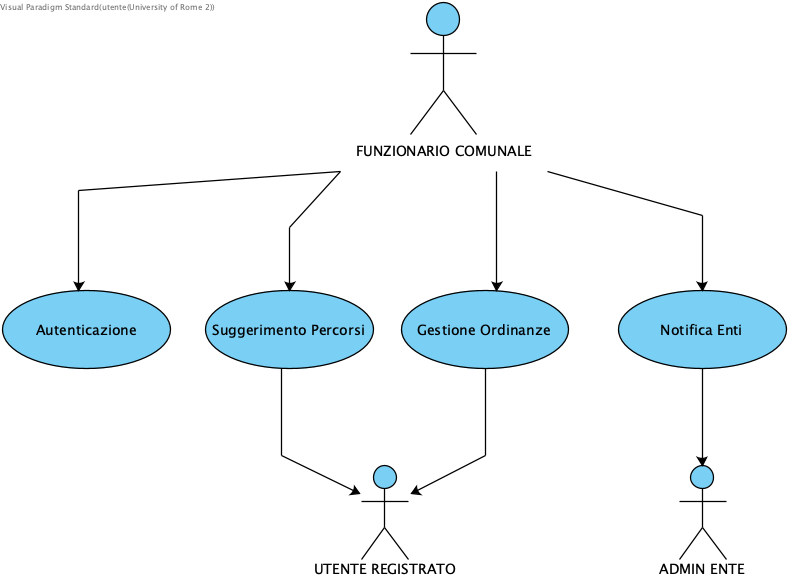
\includegraphics[width=0.7\linewidth]{UseCase/Funzionario_Comunale.png}
    \label{fig:placeholder}
\end{figure}

\subsection*{Documentazione}
\addcontentsline{toc}{subsection}{Documentazione}

\begin{center}
    Use Case: Autenticazione. 
\end{center}
Il caso d'uso Autenticazione, descrive la procedura di accesso al sistema da parte del Funzionario Comunale. \\
Attraverso l'autenticazione il sistema ricorda chi è il Funzionario Comunale, in base ai dati che ha fornito durante la Registrazione. \\
Tramite l'inserimento delle proprie credenziali, l'utente viene riconosciuto dal sistema e sblocca l'accesso a servizi appositamente per lui, più nel dettaglio, la gestione delle ordinanze di chiusura strade per eventi.

\vspace{0.5cm}

%TABELLA 
\usecasetable
{Autenticazione Funzionario}
{Accesso alle funzioni istituzionali del portale mobilità.}
{Funzionario Comunale.}
{Possesso di credenziali istituzionali.}
{1. Inserimento dati accesso. \newline 2. Validazione. \newline 3. Accesso area ordinanze e notifiche.}
{1a. Password scaduta: obbligo di rinnovo credenziali.}
{Funzionario abilitato all'inserimento di atti amministrativi.}

\begin{center}
    Use Case: Gestione Ordinanze.
\end{center}
Il caso d'uso Gestione Ordinanze, solamente relativo al profilo del Funzionario Comunale, permette l'inserimento di ordinanze rilasciate dal Comune e visibili all'interno del sistema.

\vspace{0.5cm}

%TABELLA
\usecasetable
{Gestione Ordinanze}
{Inserimento di provvedimenti comunali con impatto sulla viabilità.}
{Funzionario Comunale.}
{Autenticazione Funzionario completata.}
{1. Caricamento ordinanza. \newline 2. Definizione aree impattate. \newline 3. Invio notifiche.}
{1a. Documento non valido: il sistema richiede un formato PDF conforme.}
{Alert visibili su mappa e notifiche inviate agli enti interessati.}
\newpage

\begin{center}
    Use Case: Suggerimento Percorsi.
\end{center}
Il caso d'uso Suggerimento Percorsi, anch'esso solamente relativo al profilo del Funzionario Comunale, permette la gestione dei mezzi, ovvero le variazioni apportate ai percorsi in caso di eventi mondani.

\vspace{0.5cm}

%TABELLA 
\usecasetable
{Suggerimento Percorsi}
{Modifica dinamica dei tracciati in risposta a esigenze temporanee.}
{Funzionario Comunale.}
{Autenticazione Funzionario completata.}
{1. Identificazione area critica. \newline 2. Tracciamento percorso alternativo. \newline 3. Approvazione modifica.}
{2a. Percorso non percorribile: il sistema segnala vincoli di altezza/peso per i mezzi pesanti.}
{Ricalcolo automatico dei tempi di percorrenza e percorsi per l'utenza.}

\begin{center}
    Use Case: Notifiche Enti
\end{center}
Il caso d'uso Notifiche Enti, anch'esso solamente relativo al profilo del Funzionario Comunale. \\ 
Questa funzionalità permette a quest'ultimo di notificare agli Enti, attraverso allert automatici, deviazioni o cambiamenti sulla gestione della mobilità urbana.

\vspace{0.5cm}

% TABELLA 
\usecasetable
{Notifiche Enti}
{Comunicazione formale di variazioni della mobilità verso soggetti terzi.}
{Funzionario Comunale.}
{Autenticazione Funzionario completata.}
{1. Creazione avviso. \newline 2. Informare gli Enti \newline 3. Invio.}
{3a. Errore invio: notifica di mancata ricezione per specifici canali.}
{Enti informati e coordinati sulle variazioni del traffico urbano.}
\newpage

\section{Use Case Payment}
Infine, vengono analizzati i casi d'uso legati al Pagamento. \\ Anche qui, troviamo un diagramma UML, che ci permette di mostrare come si sviluppa il flusso. \\ 
Le tabelle che seguono servono invece a "smontare" le singole transazioni e spiegarle nel dettaglio.

\subsection*{Diagramma}
\addcontentsline{toc}{subsection}{Diagramma}
\begin{figure}[H]
    \centering
    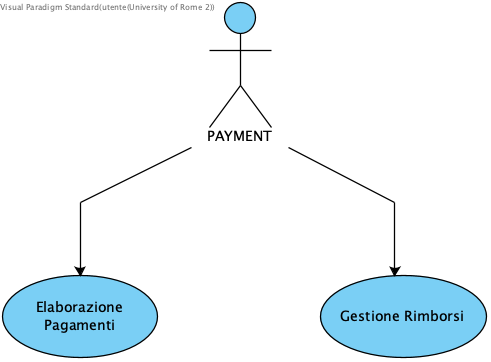
\includegraphics[width=0.6\linewidth]{UseCase/Payment.png}
    \label{fig:placeholder}
\end{figure}

\subsection*{Documentazione}
\addcontentsline{toc}{subsection}{Documentazione}

\begin{center}
    Use Case: Elaborazione Pagamenti.
\end{center}
Il caso d'uso Elaborazione Pagamenti, è solamente relativo al Payment, un attore non "umano", che gestisce i pagamenti all'interno del sistema. \\ Questa funzionalità permette al payment, attraverso un'interfaccia esterna l'elaborazione delle transizioni entranti agli Enti, in sicurezza.

\vspace{0.5cm}

%TABELLA 
\usecasetable
{Elaborazione Pagamenti}
{Gestione tecnica delle transazioni finanziarie.}
{Payment (Sistema Esterno).}
{Richiesta di acquisto avviata da un utente.}
{1. Ricezione dati transazione. \newline 2. Verifica fondi. \newline 3. Notifica esito positivo.}
{2a. Fondi insufficienti o carta scaduta: notifica errore.}
{Trasferimento fondi completato e ricevuta generata.}
\newpage

\begin{center}
    Use Case: Gestione Rimborsi.
\end{center}
Il caso d'uso Gestione Rimborsi, anch'esso solamente relativo anch'esso al Payment, permette di gestire le procedure di riborso in caso di annullamenti.

\vspace{0.5cm}

% TABELLA 
\usecasetable
{Gestione Rimborsi}
{Storno di pagamenti effettuati per servizi non usufruiti o cancellati.}
{Payment (Sistema Esterno), Admin Ente.}
{Esistenza di una transazione originale valida.}
{1. Richiesta di rimborso (automatica o manuale). \newline 2. Verifica condizioni di storno. \newline 3. Accredito fondi.}
{2a. Termini scaduti: il sistema nega il rimborso automatico.}
{Aggiornamento contabile e ripristino fondi verso l'utente.}
\newpage

\subsection*{Requisiti Funzionali}
I requisiti funzionali specificano dettagliatamente le azioni e le modalità di elaborazione dei dati che il sistema deve obbligatoriamente implementare. Sulla base degli obiettivi di digitalizzazione del contesto di Scicli, avremo i seguenti requisiti: 

\begin{table}[H]
\centering
\tiny
\renewcommand{\arraystretch}{1.4} 
\begin{tabularx}{\textwidth}{|l|l|X|X|}
\hline
\textbf{Attore} & \textbf{ID} & \textbf{Requisiti funzionali} & \textbf{Descrizione} \\ \hline

\multirow{7}{*}{Utente Registrato} & 1.1 & Autenticazione & Accede al profilo tramite credenziali per sbloccare i servizi avanzati. \\ \cline{2-4} 
 & 1.2 & Consultazione mobilità & Visualizza orari, fermate, mappe e itinerari in tempo reale. \\ \cline{2-4} 
 & 1.3 & Acquisto titoli di viaggio & Effettua l'acquisto di biglietti e abbonamenti digitali. \\ \cline{2-4} 
 & 1.4 & Prenotazione DRT & Prenota servizi di trasporto a richiesta per le frazioni e il centro. \\ \cline{2-4} 
 & 1.5 & Gestione preferiti & Salva percorsi e fermate frequenti per un accesso rapido. \\ \cline{2-4} 
 & 1.6 & Storico utente & Visualizza l'elenco dei viaggi effettuati e delle transazioni passate. \\ \cline{2-4} 
 & 1.7 & Pagamento soste & Corrisponde la tariffa per il parcheggio nelle aree a strisce blu. \\ \hline

\multirow{1}{*}{Utente Non Reg.} & 2.1 & Registrazione & Effettua una registrazione compilando un form dove inserisce un username, una password, e altri dati da utilizzare nella fase di Autenticazione \\ \cline{2-4} 
& 2.2 & Consultazione mobilità & Visualizza orari, fermate, mappe e itinerari senza necessità di registrazione. \\ \hline

% Corretto multirow a 3 perché ci sono 3 righe per il Turista
\multirow{3}{*}{Turista} & 3.1 & Consultazione Pacchetti Speciali & Consultazione di itinerari selezionati e promozioni per turisti.\\ \cline{2-4} 
 & 3.2 & Acquisto Pacchetti Speciali & Acquisto di itinerari selezionati e promozioni per turisti.\\ \hline

\multirow{5}{*}{Admin Ente} & 4.1 & Autenticazione & Accesso protetto al pannello di controllo gestionale. \\ \cline{2-4} 
 & 4.2 & Gestione corse & Crea, modifica o cancella linee, orari e frequenze dei mezzi. \\ \cline{2-4} 
 & 4.3 & Gestione flotta & Gestisce l'aggiunta o la rimozione dei mezzi monitorati. \\ \cline{2-4} 
 & 4.4 & Gestione tariffe & Configura i costi dei titoli di viaggio e le promozioni attive. \\ \cline{2-4} 
 & 4.5 & Gestione staff & Assegna gli operatori alle corse e monitora il servizio. \\ \hline

\multirow{4}{*}{Operatore} & 5.1 & Autenticazione & Accesso al pannello di controllo degli autisti. \\ \cline{2-4} 
 & 5.2 & Gestione corse DRT & Riceve e accetta le assegnazioni per il trasporto a chiamata. \\ \cline{2-4} 
 & 5.3 & Stato servizio & Segnala l'inizio, la fine o eventuali anomalie/ritardi. \\ \cline{2-4} 
 & 5.4 & Verifica prenotazioni & Visualizza la lista dei passeggeri prenotati per la tratta. \\ \hline

\multirow{4}{*}{Funzionario Comunale} & 6.1 & Autenticazione & Accesso autorizzato per la gestione della viabilità cittadina. \\ \cline{2-4} 
 & 6.2 & Gestione ordinanze & Inserisce avvisi di chiusura strade per eventi o manutenzione. \\ \cline{2-4} 
 & 6.3 & Suggerimento percorsi & Imposta deviazioni e itinerari alternativi per i mezzi. \\ \cline{2-4} 
 & 6.4 & Notifica enti & Invia alert automatici ai gestori per variazioni urgenti. \\ \hline

\multirow{2}{*}{Payment (System)} & 7.1 & Elaborazione pagamenti & Interfaccia esterna per processare le transazioni in sicurezza. \\ \cline{2-4} 
 & 7.2 & Gestione rimborsi & Gestisce le procedure di storno in caso di annullamento. \\ \hline

\end{tabularx}
\end{table}
\newpage

\subsection*{Requisiti Non Funzionali}
I requisiti non funzionali descrivono le caratteristiche qualitative, i vincoli tecnici e i livelli di servizio del software. 
\\
Per il nostro software, stabiliamo i seguenti parametri:

\begin{table}[h!]
\centering
\small
\renewcommand{\arraystretch}{1.5}
\begin{tabularx}{\textwidth}{|l|X|}
\hline
\textbf{Requisito} & \textbf{Descrizione} \\ \hline
\textbf{Performance} & Il sistema deve garantire il caricamento delle mappe e degli orari in maniera rapida per assicurare un'esperienza fluida. \\ \hline

\textbf{Scalabilità} & Il sistema deve permettere l'aggiunta di nuovi enti di trasporto e deve supportare un incremento del traffico gestito con l'integrazione di ulteriori API di mobilità (es. Google Maps Platform, TomTom API) senza richiedere una ristrutturazione del codice esistente. \\ \hline

\textbf{Portabilità} & L'applicazione, sviluppata con il framework React Native, deve garantire la piena compatibilità con i sistemi operativi Android e iOS. L'interfaccia deve adattarsi correttamente a diverse risoluzioni e dimensioni di schermo degli smartphone. \\ \hline

\textbf{Affidabilità} & Il sistema deve operare correttamente nel 99\% dei casi, garantendo la continuità dei servizi di trasporto essenziali. In caso di errore nel processo di pagamento o nella prenotazione, il software deve fornire feedback chiari e gestire il ripristino dello stato precedente per evitare perdite di dati o transazioni duplicate. \\ \hline

\textbf{Manutenibilità} & La struttura deve consentire interventi di manutenzione rapidi e l'aggiornamento semplificato dei database relativi a orari e tariffe. Il codice deve essere documentato per facilitare il passaggio di consegne e futuri sviluppi incrementali da parte dell'amministrazione comunale. \\ \hline

\textbf{Disponibilità} & Le funzionalità di mobilità devono essere operative per il 99.5\% del tempo, specialmente durante le fasce orarie di servizio dei mezzi pubblici e delle navette turistiche. Il monitoraggio delle chiusure stradali deve essere garantito h24 per fornire sempre percorsi aggiornati. \\ \hline

\textbf{Usabilità} & L'interfaccia deve essere intuitiva per un pubblico eterogeneo (residenti e turisti). Il design deve supportare la multilingua (italiano/inglese). L'obiettivo è minimizzare il tasso di errore dell'utente durante le varie  prenotazioni. \\ \hline

\textbf{Sicurezza} & La gestione dei dati sensibili, della cronologia degli spostamenti e delle transazioni finanziarie deve essere protetta tramite crittografia. L'accesso alle funzionalità di gestione (Admin Ente e Funzionario) deve essere regolato da un sistema di autenticazione robusto per prevenire accessi non autorizzati. \\ \hline
\end{tabularx}
\end{table}